\documentclass[twocolumn]{article}

\usepackage[margin=1in]{geometry}
\usepackage{amsmath}
\usepackage{booktabs}
\usepackage{listings}
\usepackage{wrapfig}
\usepackage{epsfig}
\usepackage{float}
\usepackage{graphicx}
\usepackage{fancyhdr}
\usepackage{hyperref}

\pagestyle{fancy}
\lhead{Francisco Rivera}
\rhead{Numerical Exploration of Local Volatility}


\usepackage{color}
\definecolor{lgray}{gray}{0.95}
\definecolor{mygreen}{rgb}{0,0.6,0}
\definecolor{mygray}{rgb}{0.5,0.5,0.5}
\definecolor{mymauve}{rgb}{0.58,0,0.82}
\lstset{ %
  backgroundcolor=\color{lgray},   % choose the background color; you must add \usepackage{color} or \usepackage{xcolor}; should come as last argument
  basicstyle=\ttfamily\footnotesize,        % the size of the fonts that are used for the code
  breakatwhitespace=false,         % sets if automatic breaks should only happen at whitespace
  breaklines=true,                 % sets automatic line breaking
  commentstyle=\color{mygreen},    % comment style
  deletekeywords={...},            % if you want to delete keywords from the given language
  escapeinside={\%*}{*)},          % if you want to add LaTeX within your code
  extendedchars=true,              % lets you use non-ASCII characters; for 8-bits encodings only, does not work with UTF-8
  keepspaces=true,                 % keeps spaces in text, useful for keeping indentation of code (possibly needs columns=flexible)
  keywordstyle=\color{blue},       % keyword style
  language=Python,                 % the language of the code
  morekeywords={*,...},            % if you want to add more keywords to the set
  numbers=left,                    % where to put the line-numbers; possible values are (none, left, right)
  numbersep=5pt,                   % how far the line-numbers are from the code
  numberstyle=\tiny\color{mygray}, % the style that is used for the line-numbers
  rulecolor=\color{black},         % if not set, the frame-color may be changed on line-breaks within not-black text (e.g. comments (green here))
  showspaces=false,                % show spaces everywhere adding particular underscores; it overrides 'showstringspaces'
  showstringspaces=false,          % underline spaces within strings only
  showtabs=false,                  % show tabs within strings adding particular underscores
  stepnumber=1,                    % the step between two line-numbers. If it's 1, each line will be numbered
  stringstyle=\color{mymauve},     % string literal style
  tabsize=2,	                   % sets default tabsize to 2 spaces
}

\begin{document}

\onecolumn

\title{A Numerical Exploration of the Local Volatility Model for Option Pricing}
\author{Francisco Rivera \and Kevin Chen}
\date{\today}

\maketitle

\begin{abstract}
In Nobel-prize winning work, Black, Merton, and Scholes developed a model to
price options. The tractability of the model revolutionized options pricing and
allowed for the derivatives to become widely traded. However, the
predictions of the model run counterfactual to empirically observed prices. In
this paper, we consider a generalization to the Black-Scholes model, the
local-volatility model. This generalization gives us more degrees of freedom to
fit the prices we observe. With the additional expressiveness, however, come
numerical complications. Black-Scholes requires fitting only a single number
known as the \emph{implied volatility}, but the local volatility model requires
fitting an entire multi-dimensional function. We explore these complications and
arrive at solutions that are assessed for numerical stability and accuracy to
price out-of-sample options.
\end{abstract}

\tableofcontents

\twocolumn

\newpage

\section{Background}
\label{sec:background}

\subsection{Options Terminology}
\label{subsec:terminology}

Before delving into the theoretical and numerical results, we briefly summarize
options terminology. An option is a derivative on some asset, henceforth called
the \emph{underlying}---i.e.\ it's value is \emph{derived} from the value of the
underlying. The owner of a call/put option has the right but not the obligation
to buy/sell the underlying asset at a given price at some date in the future.

The price at which the holder of the option can buy/sell is called the
\emph{strike price}, denoted $K$. Invoking the right to buy/sell is called
\emph{exercising} the option. The last time at which the holder can exercise is
called the \emph{expiry}, denoted as time $T$. The value of the underlying asset
at time $t$ is denoted as $S_t$. 

The payoff of a call option at expiry is thus given by,
\[ \max(S_T - K, 0) \]
because the owner will only exercise it if the underlying is worth more than the
strike price.

\begin{center}
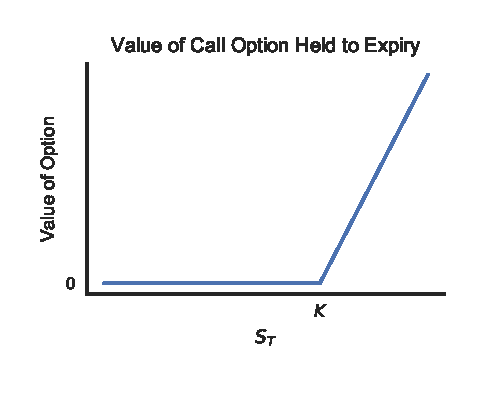
\includegraphics{figs/calloptpayoff}
\end{center}

The payoff of a put option is simililarly,
\[ \max(K-S_T, 0) \]
and the payoff curve looks like,

\begin{center}
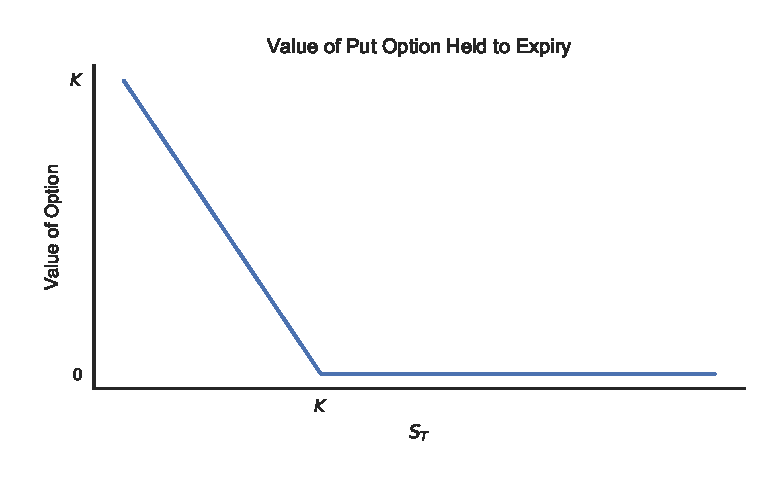
\includegraphics{figs/putoptpayoff}
\end{center}

\subsection{Risk-Neutral Pricing}

The value of an option at expiry is easily observable and displayed in the
figures in Section \ref{subsec:terminology}. However, before time $T$, the
value of $S_T$ is a random variable. Asset pricing (change of measure) theorems
allow us to write the value of a call option as the discounted expectation of
the payoff under what we call the risk-neutral distribution,
\[ C(T,K) = e^{-rT} \int_K^\infty (S - K)
\underbrace{\phi(T,S)}_\text{risk-neutral PDF} \, dS.\]
However, in order to make any progress beyond this, we need to make a further
assumption about what this risk-neutral distribution looks like.

\subsection{Black-Scholes Model}
The Black-Scholes model makes one such assumption by writing how the asset
diffuses over time. In particular, the Black-Scholes model treates the asset
price as a geometric Brownian motion such that,
\[ \frac{dS}{S} = r dt + \sigma dW \]
where $W$ is Brownian motion and $\sigma$ is a constant value called the implied
volatility. 

This forces the risk-neutral distribution to be log-normal and makes
finding the price analytically tractable. In particular, since the only pricing
input into this model that we do not observe is the implied volatility, we can
quote price as a function of implied volatility (e.g. an option is said to cost
$\sigma=16\%$ if its price is consistent with the price the Black-Scholes model
would predict if $\sigma=16\%$).

Thus, Black-Scholes predicts that if $\sigma$ is indeed a constant, then for any
option written on the same underlying (regardless of strike price or expiry),
that the implied volatility will be (approximately) constant. However, this is
directly counterfactual to the options prices that we observe. For example,
looking at the prices of AAPL options that expire on January 2018 retrieved on
November 20$^\text{th}$, 2017 from Yahoo Finance, we get the following curve

\begin{center}
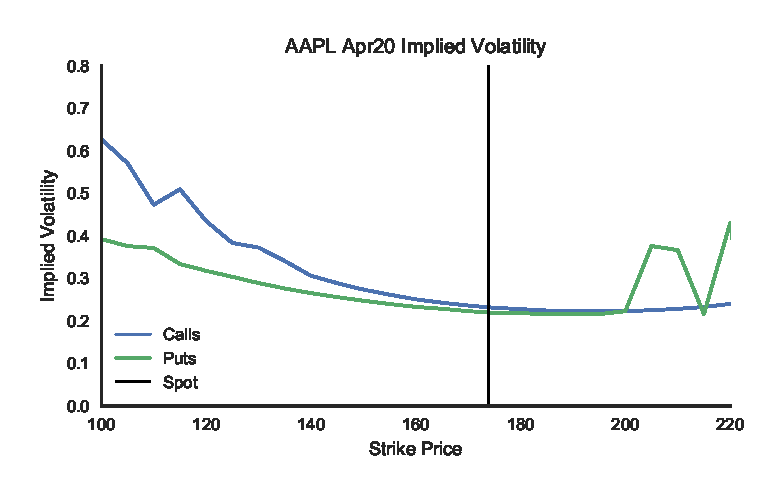
\includegraphics{figs/aapliv}
\end{center}

While the data is noisy, particularly for deep-in-the money puts
which are hardly ever traded, the graph is unmistakably not constant. Moreover,
AAPL is not an exception: most graphs of implied volatility versus strike have a
similar shape. These deviations from Black-Scholes also correspond to
intuitive qualitative ideas. If the price of AAPL has just plunged 50\%, it is
palatable to think there is a lot of investor uncertainty, and that the future
price of AAPL will diffuse with higher volatility than if it is just up 5\%.
Thus, the assumption of constant $\sigma$ is suspect.

\section{Local Volatility Theory}

\section{Pricing with Local Volatility}

\section{Fitting Local Volatility}

\section{Conclusions}

\end{document}
